\documentclass{beamer}

\usepackage{helvet}
\usepackage{hyperref, graphicx}
\usepackage{amsthm}
\usepackage{etoolbox}

\usetheme{default}
\setbeamertemplate{navigation symbols}{}
\AtBeginSection[ ]
{
\begin{frame}{Outline}
    \tableofcontents[currentsection]
\end{frame}
}

% Default fixed font does not support bold face
\DeclareFixedFont{\ttb}{T1}{txtt}{bx}{n}{11} % for bold
\DeclareFixedFont{\ttm}{T1}{txtt}{m}{n}{12}  % for normal - use in headings

% Custom colors
\usepackage{color}
\definecolor{TUGray}{RGB}{101,101,137}
\definecolor{TUBlack}{RGB}{30,0,0}
\definecolor{mygreen}{RGB}{45,111,63}
\definecolor{keywords}{RGB}{205,114,0}
\definecolor{comments}{RGB}{181,51,139}
\definecolor{strings}{RGB}{58,144,81}
\definecolor{numeric}{RGB}{66,110,176}
\definecolor{linos}{rgb}{0.4,0.4,0.4}
\definecolor{links}{rgb}{0,0.4,0.75}

\definecolor{bggray}{RGB}{232, 233, 235}

\usecolortheme[named=mygreen]{structure}
\setbeamercolor{normal text}{fg=TUBlack}\usebeamercolor*{normal text}

\setbeamercolor{codecol}{fg=TUGray!25!black,bg=bggray}

\hypersetup{colorlinks, linkcolor=links, urlcolor=links}

\usepackage[T1]{fontenc}
\usepackage[sfdefault,scaled=.85]{FiraSans}
\usepackage{newtxsf}

\usepackage{listings}

\newtoggle{InString}{}% Keep track of if we are within a string
\togglefalse{InString}% Assume not initally in string

\newcommand\digitstyle{\color{numeric}}
\makeatletter
\newcommand{\ProcessDigit}[1]
{%
  \ifnum\lst@mode=\lst@Pmode\relax%
   {\digitstyle #1}%
  \else
    #1%
  \fi
}
\makeatother

\lstset{literate=%
    {0}{{{\ProcessDigit{0}}}}1
    {1}{{{\ProcessDigit{1}}}}1
    {2}{{{\ProcessDigit{2}}}}1
    {3}{{{\ProcessDigit{3}}}}1
    {4}{{{\ProcessDigit{4}}}}1
    {5}{{{\ProcessDigit{5}}}}1
    {6}{{{\ProcessDigit{6}}}}1
    {7}{{{\ProcessDigit{7}}}}1
    {8}{{{\ProcessDigit{8}}}}1
    {9}{{{\ProcessDigit{9}}}}1
	{<=}{{\(\leq\)}}1
	{>=}{{\(\geq\)}}1,
	% morestring=[b]",
    % morestring=[b]',
    % morecomment=[l]//,
}

% Python style for highlighting
\newcommand\pythonstyle{\lstset{
language=Python,
basicstyle=\ttfamily\tiny,
numbers=left,
numberstyle=\tiny\color{linos},
morekeywords={self},              % Add keywords here
keywordstyle=\tiny\color{keywords},
commentstyle=\it\tiny\color{comments},    % Custom highlighting style
stringstyle=\tiny\color{strings},
xleftmargin=18pt,
xrightmargin=4pt,
aboveskip=0pt,
belowskip=0pt,
escapeinside={(*@}{@*)},
frame=l,                         % Any extra options here
showstringspaces=false,
keepspaces=true
}}

% Python environment 
\lstnewenvironment{python}[1][]
{
	\pythonstyle
	\lstset{
	#1
	}
}
{}

% wrap the Python environment
\newenvironment{codeblock}
    {\hfill\begin{beamerboxesrounded}[lower=codecol, width=0.8\textwidth]
    \medskip

    }
    { 
    \end{beamerboxesrounded}\hfill
    }

\theoremstyle{example}
\newtheorem{question}{Question}

\newcommand{\ct}[1]{\lstinline[language=Python]!#1!}
\newcommand{\ttt}[1]{{\small\texttt{#1}}}
\newcommand{\lsitem}[2]{\ttt{{#1}[}\ct{#2}\ttt{]}}

\author{Chris Cornwell}
\date{Feb 4, 2025}
\title{The Random package, Defining Custom Functions}

\begin{document}

\begin{frame}
\titlepage
\end{frame}

\begin{frame}
\frametitle{Outline}
\tableofcontents
\end{frame}

\section{Random functions in NumPy}

%%%%
\begin{frame}[fragile]
\frametitle{The {\ttm random} module in NumPy}
From documentation: Within NumPy is the package \ttt{random} which ``implments pseudo-random number generators\ldots with the ability to draw samples from a variety of probability distributions.''
%\pause
\begin{enumerate}
    \item Uniform discrete: to sample \ttt{m} numbers from the uniform distribution on the integers in \ttt{range(n)}, use the function \ttt{np.random.randint(n, size=m)}. 
    \begin{itemize}
        \item An optional additional integer in the arguments: give a lower bound.\footnote{The default lower end is 0, to sample between 0 and \ttt{n-1}.}
        \item If size argument not given, just one number returned. If the \ttt{size=m} is given, returns a NumPy array.
    \end{itemize}
\end{enumerate}

%\pause 
\begin{codeblock}

\begin{python}
    # 20 integers, each equally likely, between 1 and 10
    np.random.randint(1, 11, size=20)
\end{python}

\end{codeblock}

%\pause
\begin{enumerate}
    \item[] Commands above will sample with replacement.
    \begin{itemize}
        \item To sample without replacement, use argument \ttt{replace=}{\color{numeric}\ttt{False}}.
    \end{itemize}
\end{enumerate}

\end{frame}

%%%%
\begin{frame}[fragile]
\frametitle{The {\ttm random} module in NumPy}

\begin{enumerate}
    \setcounter{enumi}{1}
    \item Uniform continuous: to sample \ttt{m} floats in the interval \ttt{[a, b)}, use the function \ttt{np.random.uniform(a, b, size=m)}.
    \begin{itemize}
        %\pause
        \item The defaults for the left \& right endpoints are 0 and 1. This means that \ttt{np.random.uniform(size=m)} will sample from the unit interval.
        \item An alternative: \ttt{np.random.random(size=m)}. Only samples from the unit interval, but, can get samples from \ttt{[a,b)} by multiplying and adding (below).
    \end{itemize}
\end{enumerate}

\vspace*{12pt}
%\pause
\begin{codeblock}

\begin{python}[numbers=none]
(b-a)*np.random.random(size=m) + a
\end{python}

\end{codeblock}

\end{frame}

%%%%
\begin{frame}[fragile]
    \frametitle{The {\ttm random} module in NumPy}
    
    \begin{enumerate}
        \setcounter{enumi}{1}
        \item Uniform continuous: to sample \ttt{m} floats in the interval \ttt{[a, b)}, use the function \ttt{np.random.uniform(a, b, size=m)}.
        \item Normal distribution: to sample \ttt{m} floats from the normal distribution, with mean \ttt{mu} and standard deviation \ttt{sigma}, use the function \ttt{np.random.normal(mu, sigma, size=m)}
        \begin{itemize}
            \item The two arguments for the mean and standard deviation have default 0 and 1, respectively.
            \item Not uncommon to use the \emph{keywords} for these arguments,\footnote{Using keyword makes the argument not \emph{positional} anymore; arguments coming after it must have keyword too.} as in 
            \begin{center}\ttt{np.random.normal(loc=mu, scale=sigma, size=m)}\end{center}
        \end{itemize}
    \end{enumerate}

    %\pause
    Larger the sample, the closer the sample distribution should be to the theoretical distribution. Can we display this in a plot?
\end{frame}
    
%%%%
\begin{frame}[fragile]
\frametitle{Visualizing the distribution}
Say that we are using the uniform distribution on the interval $[a,b)$. For a small subinterval of width $\delta$, we have probability $\delta\frac{1}{b-a}$ of getting a sample in that interval.

%\pause
Consequence: if plot (normalized) histogram of sample over the interval $[a,b]$, being close to the distribution means bars are close to height $1/(b-a)$, on average. Below is a histogram from a sample of size 50, from \ttt{uniform(0, 5)}.

\begin{codeblock}

\begin{python}
xx = np.linspace(0,5)
sample = np.random.uniform(0, 5, size=50)
# will also plot horizontal line at height 1/(b-a)
plt.plot(xx, [1/5]*len(xx), color='black')
# "density=True" below -> divide height of each bar by number of samples
plt.hist(sample, bins=10, density=True)
plt.show()
\end{python}

\end{codeblock}

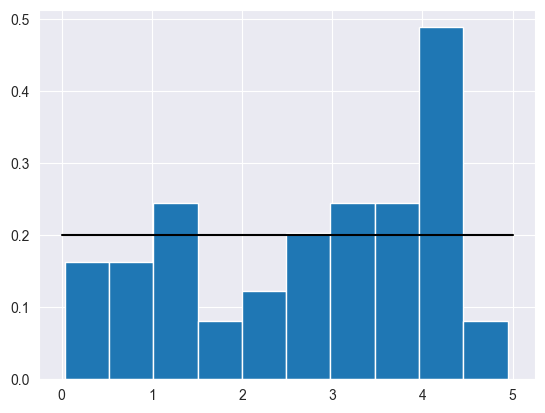
\includegraphics[width=0.7\textwidth]{histogram_of_sample1.png}

\end{frame}

%%%%
\begin{frame}[fragile]
\frametitle{Visualizing the distribution}

A larger sample size will (on average) give a sample distribution that is closer to the \emph{true} one. For example, by changing our previous code so that the sample size is 5000, we can see the sample distribution get much closer.

%\pause
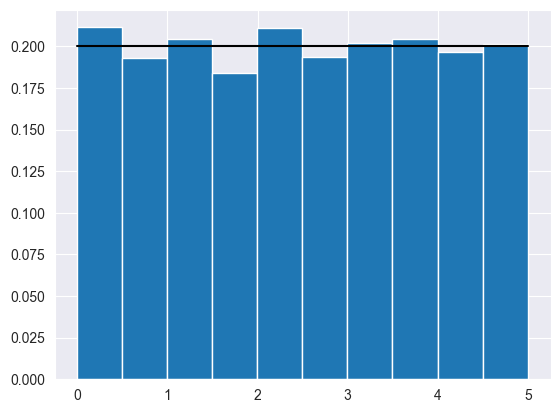
\includegraphics[width=0.7\textwidth]{histogram_of_sample2.png}

\end{frame}

%%%%
\begin{frame}[fragile]
\frametitle{Visualizing the normal distribution}
If using the normal distribution, with mean $\mu$ and st.deviation $\sigma$, the density function is \[p(x) = \frac{1}{\sqrt{2\pi\sigma^2}}e^{-\frac{(x-\mu)^2}{2\sigma^2}}.\]

Consequence: a histogram of a sample being close to the distribution means top of bars are close to graph of $p(x)$. To make the histogram, can do following.\footnote{Doubled the sample size and the number of bins, due to greater variability in the pdf of the distribution.}

%\pause

\begin{codeblock}

\begin{python}
xx = np.linspace(-3,3)
sample = np.random.normal(0, 1, size=100)
plt.hist(sample, bins=20, density=True)
plt.show()
\end{python}

\end{codeblock}

%\pause
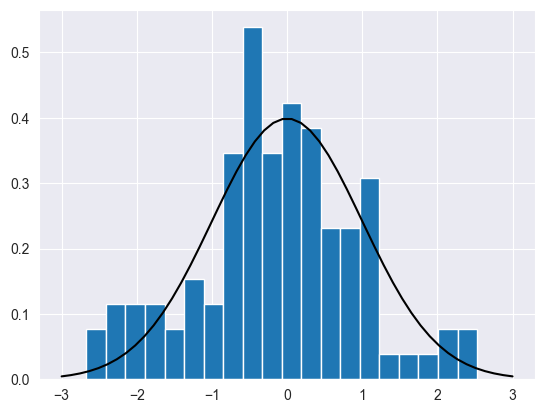
\includegraphics[width=0.7\textwidth]{histogram_of_sample3.png}

\end{frame}

%%%%

\begin{frame}[fragile]
\frametitle{Visualizing the normal distribution}
    
Again, about the normal distribution
    
%\pause
%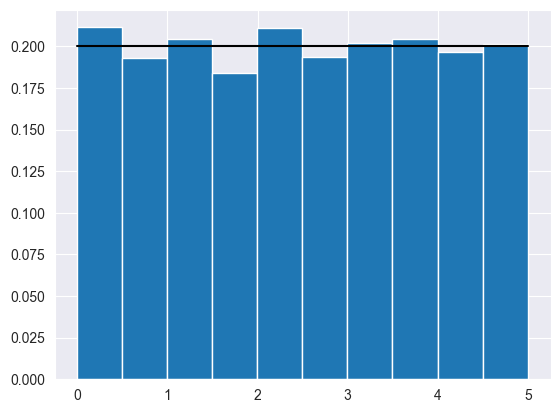
\includegraphics[width=0.7\textwidth]{histogram_of_sample2.png}
    
\end{frame}

% from on getting matrix entries

% shuffling a random permutation
    
\section{Defining custom functions}

%%%%
\begin{frame}[fragile]
\frametitle{Constructing special matrices}
Some types of matrices are used a lot; would be cumbersome to always write the row lists ourselves (e.g., in a $100\times100$ matrix).
    
    %pause
    \begin{itemize}
        \item[] \textbf{Zero matrix}: The command \ttt{np.zeros((m, n))} constructs an $m\times n$ matrix with all entries equal to zero.
        %\pause
        \item[] \textbf{Diagonal matrix}: If \ttt{d} is a 1d array of length $n$, the command \ttt{np.diag(d)} constructs an $n\times n$ diagonal matrix which has \ttt{d} as its diagonal entries.
        %\pause
        \item[] \textbf{Identity matrix}: The command \ttt{np.eye(n)} constructs the $n\times n$ identity matrix.
    \end{itemize}
    
%pause
\textbf{Extracting part of matrix:} May want to get part of a matrix. To get a submatrix from consecutive rows and columns, use slicing. %\pause
Also, here are functions that return part of the matrix (other entries being set to \ttt{0}).%\footnote{Can use a \emph{method} for last one: \ttt{A.diagonal()} returns the same as \ttt{np.diag(A)}.} 

\begin{codeblock}

\begin{python}
# return lower triangular part (at or below the diagonal)
np.tril(A)
# return upper triangular part (at or above the diagonal)
np.triu(A)
# return the diagonal of A
np.diag(A)
\end{python}

\end{codeblock}
\end{frame}

%%%%
\begin{frame}
\frametitle{Using NumPy for linear algebra}
In addition to the product operations on arrays, NumPy has a library (\ttt{linalg}) with many functions for linear algebra. 

%\pause
Examples: 
\begin{enumerate}
    \item If $M$ is a square matrix, can compute $\det(M)$ with the command \ttt{np.linalg.det(M)}.
    %\pause
    \item When $M$ is invertible, can compute $M^{-1}$ with the command \ttt{np.linalg.inv(M)}.
    %\pause
    \item If $M$ is a square matrix, can compute eigenvalues and eigenvectors with \ttt{np.linalg.eig(M)}. 
\end{enumerate}

%\pause
There are many other linear algebra functions. Some are only implemented for square matrices (and perhaps only invertible ones), even though it would make sense to have them work more generally {--} for example, \ttt{np.solve(A, b)} only solves the system $A\mathbf{x} = b$ if \ttt{A} is a square invertible matrix.
\end{frame}

%%%%
\begin{frame}[fragile]
\frametitle{Solving a linear system \& Errors}
To solve $A\mathbf{x} = \mathbf{b}$, with a square invertible matrix \ttt{A} and vector \ttt{b} of the right size, you can use \ttt{np.linalg.solve(A, b)}.

%\pause
What happens when \ttt{A} is not square? Execute the following code in Python.

\begin{codeblock}

\begin{python}
    A = np.array([[1, 2, 3], [1, 4, -1]])
    b = np.array([1, -5])
    # system has solution x = [0, -1, 1]
    # but next line raises an error
    x = np.linalg.solve(A, b)
\end{python}

\end{codeblock}

%\pause
A message is generated about the error. It gives you helpful information, if it can. In this case, it is a \ttt{LinAlgError} with the message \ttt{Last 2 dimensions of the array must be square}.

%\pause
Spend time trying to use error messages to understand issues in your code. Also, have healthy skepticism about AI assistants. They hallucinate; error messages don't.\footnote{While writing this slide, Github Copilot suggested I write that it would be a \ttt{ValueError} from \emph{mismatched dimensions}: rows of \ttt{A} being size \ttt{(3,)} and the vector \ttt{b} being size \ttt{(2,)}.}
\end{frame}

\section{Broadcasting and efficient operations}
%%%%
\begin{frame}[fragile]
\frametitle{Broadcasting, universal functions}
Say that you have a 1d array and you want to make array with square root the entries. 
\begin{itemize}
    \item[] First thought: use a loop, taking square root (and assigning) as you go through items in the array.
\end{itemize}

NumPy has an efficient way to handle it, called \emph{broadcasting}. If \ttt{v} is your array, then you can simply type 

\begin{codeblock}

\begin{python}[numbers=none]
sqrt_v = np.sqrt(v)
\end{python}

\end{codeblock}

\begin{itemize}
    \item[] The function \ttt{np.sqrt()} takes the square root of each entry in \ttt{v}; you don't need to write the for loop.\footnote{Technically, there's a for loop in the background, but it happens in C and works much faster.}
\end{itemize}
Functions that work on arrays this way are quite common in NumPy. They are called {\ttb ufuncs} (universal functions).

%\pause
Other examples of ufuncs in NumPy: 
    \begin{itemize}
        \item[] \ttt{np.abs()}, \ttt{np.sum()}, \ttt{np.maximum()}, \ttt{np.minimum()}, \ttt{np.exp()}, \ttt{np.log()}.
    \end{itemize}
\end{frame}

\begin{frame}
\frametitle{More on broadcasting}
Many basic operations with NumPy arrays use broadcasting. Here are a few examples with an array \ttt{v}.
\begin{enumerate}
    \item To add the same scalar, say \ct{3}, to every array entry: type \ttt{v+3}.
    \item To multiply every entry by \ct{3}: type \ttt{3*v}.
    %\pause
    \item To square every entry of an array: type \ttt{v**2}.
    \item To multiply \ttt{v} by another array \ttt{w}, entry-wise\footnote{In mathematics, this product on vectors is called the Hadamard product.}: type \ttt{v*w}.
\end{enumerate}

%\pause
Everything mentioned here works just as well on matrices (2d arrays), and generally on any \ttt{n}d array (higher order tensors).

\vspace*{12pt}
%\pause
Exercise. \newline
Write out code that uses broadcasting to create a $100\times 100$ matrix where all non-diagonal entries are $-1$ and all diagonal entries are $2$.
\end{frame}

%%%%
\begin{frame}[fragile]
\frametitle{Experiment with runtime for universal function}
To check the efficiency of broadcasting, use the \ttt{time} package. Beforehand, make sure that you imported both \ttt{numpy} and \ttt{time} (see slide in first section).

%\pause
Something simple: from a large identity matrix, we will get the exponential of the matrix (apply the function $e^x$ to every entry).

%\pause
First, we use a \ttt{for} loop. Run the code below in your Jupyter notebook.

\begin{codeblock}

\begin{python}
id_matrix = np.eye(1000)
exp_matrix = np.zeros((1000, 1000))
start = time.time()
for i in range(1000):
    for j in range(1000):
        exp_matrix[i,j] = np.exp(id_matrix[i,j])
end = time.time()
print(f"Seconds taken: {end-start}.")
\end{python}

\end{codeblock}

\vspace*{12pt}
%\pause
\begin{itemize}
    \item[] The output gives the number of seconds to run the computation. The exact time will vary based on your computer. Mine took around 0.55 seconds.
\end{itemize}
\end{frame}

%%%%
\begin{frame}[fragile]
\frametitle{Experiment with runtime for universal function}
Now, we will use broadcasting to compute the exponential of the identity matrix.

%\pause
Run the following code in your Jupyter notebook.

\begin{codeblock}

\begin{python}
id_matrix = np.eye(1000)
exp_matrix = np.zeros((1000, 1000))
start = time.time()
exp_matrix = np.exp(id_matrix)
end = time.time()
print(f"Seconds taken: {end-start}.")
\end{python}

\end{codeblock}

\vspace*{12pt}
%\pause
\begin{itemize}
    \item[] Again, the output is the number of seconds of runtime. For this approach with \ttt{np.exp()}, my computer took around 0.0045 seconds. That is over 100 times faster than writing the loop!
\end{itemize}
\end{frame}

\end{document}